\documentclass{beamer}

%\usetheme{AnnArbor}
%\usetheme{Antibes}
%\usetheme{Bergen}
%\usetheme{Berkeley}
%\usetheme{Berlin}
%\usetheme{Boadilla}
%\usetheme{boxes}
%\usetheme{CambridgeUS}
%\usetheme{Copenhagen}
%\usetheme{Darmstadt}
%\usetheme{default}
%\usetheme{Frankfurt}
%\usetheme{Goettingen}
%\usetheme{Hannover}
%\usetheme{Ilmenau}
%\usetheme{JuanLesPins}
%\usetheme{Luebeck}
\usetheme{Madrid}
%\usetheme{Malmoe}
%\usetheme{Marburg}
%\usetheme{Montpellier}
%\usetheme{PaloAlto}
%\usetheme{Pittsburgh}
%\usetheme{Rochester}
%\usetheme{Singapore}
%\usetheme{Szeged}
%\usetheme{Warsaw}
\usepackage{beamerthemesplit} % new 
\setbeamertemplate{items}[rectangle]
\setbeamertemplate{navigation symbols}{}
\usepackage{graphicx} 
\usepackage[labelformat=empty]{caption} % pas de "Figure: "
\usepackage{textcomp}
\usepackage{makeidx}
\usepackage{amsfonts}
\usepackage{amsmath,amssymb,latexsym}
\usecolortheme[RGB={21, 101, 178}]{structure} 
\usepackage{color}
\usepackage[utf8]{inputenc}
\usepackage{listings}
\graphicspath{ {images/} }
\usepackage{listings}
\lstset{language=Java,
                basicstyle=\footnotesize\ttfamily,
                keywordstyle=\footnotesize\color{blue}\ttfamily,
}
\usepackage{color}


\lstset{%
  basicstyle=\scriptsize\sffamily,%
  commentstyle=\footnotesize\ttfamily,%
  frameround=trBL, frame=single, breaklines=true,
  showstringspaces=false, numbers=left, numberstyle=\tiny,
  numbersep=10pt, keywordstyle=\bf } \newcommand{\ssubtitle}[1]{%
  \posttitle{%
    \par\end{center}
  \begin{center}\large#1\end{center}
  \vskip0.5em}%
}

% java lst color
\definecolor{javared}{rgb}{0.6,0,0} % for strings
\definecolor{javagreen}{rgb}{0.25,0.5,0.35} % comments
\definecolor{javapurple}{rgb}{0.5,0,0.35} % keywords
\definecolor{javadocblue}{rgb}{0.25,0.35,0.75} % javadoc
\lstset{language=java, keywordstyle=\color{javapurple}\bfseries,
  stringstyle=\color{javared}, commentstyle=\color{javagreen},
  morecomment=[s][\color{javadocblue}]{/**}{*/}, tabsize=4}

\definecolor{rltred}{rgb}{0.75,0,0}
	\definecolor{rltgreen}{rgb}{0,0.5,0}
	\definecolor{oneblue}{rgb}{0.06,0.04,0.9}
	\definecolor{marron}{rgb}{0.64,0.16,0.16}
	\definecolor{forestgreen}{rgb}{0.13,0.54,0.13}
	\definecolor{purple}{rgb}{0.62,0.12,0.94}
	\definecolor{dockerblue}{rgb}{0.11,0.56,0.98}
	\definecolor{freeblue}{rgb}{0.25,0.41,0.88}
	\definecolor{myblue}{rgb}{0,0.2,0.4}

\title{Memory Access Management with LLVM and OpenCL}

\author{Mohammed Yassine Jazouani \\
jazouani@gmail.com \\
Université Grenoble Alpes, Grenoble\\
\\ \\
Supervised by: \\
Ylies Falcone, Brice Videau \\
and Jean-Fran\c{c}ois Mehaut\\}
% - Give the names in the same order as the appear in the paper.
% - Use the \inst{?} command only if the authors have different
%   affiliation.

% - Use the \inst command only if there are several affiliations.
% - Keep it simple, no one is interested in your street address.

\date{LLVM - June, 16th 2015}
% - Either use conference name or its abbreviation.
% - Not really informative to the audience, more for people (including
%   yourself) who are reading the slides online

\subject{Theoretical Computer Science}
% This is only inserted into the PDF information catalog. Can be left
% out. 

% If you have a file called "university-logo-filename.xxx", where xxx
% is a graphic format that can be processed by latex or pdflatex,
% resp., then you can add a logo as follows:

% \pgfdeclareimage[height=0.5cm]{university-logo}{university-logo-filename}
% \logo{\pgfuseimage{university-logo}}

% Delete this, if you do not want the table of contents to pop up at
% the beginning of each subsection:
\AtBeginSection[]
{
  \begin{frame}<beamer>{Summary}
    \tableofcontents[currentsection, hideallsubsections]
  \end{frame}
}

\setbeamertemplate{footline}{%
\hfill\usebeamertemplate***{navigation symbols}
\hspace{1cm}\insertframenumber{}/\inserttotalframenumber}

% Let's get started
\begin{document}

\begin{frame}
  \titlepage
\end{frame}

\begin{frame}{Summary}
  \tableofcontents[hideallsubsections]
  % You might wish to add the option [pausesections]
\end{frame}


% Section and subsections will appear in the presentation overview
% and table of contents.

%%%%%%%%%%%%%%%%%%%%%%%%%%%%%%%%%%%%%%%%%%%%%%%%%%%%%%%%%%%%%%%%%%%%%%%%%%%%%%%%%%%%%
%%%%%%%%%%%%%%%%%%%%%%%%%%%%%%%%%%%%%%%%%%%%%%%%%%%%%%%%%%%%%%%%%%%%%%%%%%%%%%%%%%%%%
\section{Introduction}

\begin{frame}{Context}
\subsection{Context}
\begin{itemize}
\item Computing devices opt for parallel programming
\item Shared memory management problem
\item Tool capable to give enough information concerning the memory to the developer to avoid these problems
\item Existing tools: 
    \begin{itemize}
    \item Implemented for LLVM: AddressSanitizer, MemorySanitizer, ThreadSanitizer
    \item Used on simulated environments: Symbolic OpenCL, OCLgrind
    \end{itemize}
\end{itemize}
\end{frame}

\begin{frame}{Problem}
\subsection{Problem}
\begin{itemize}
\item Compile time: syntax, typechecking and compiler errors
\item Runtime: only division by zero, deferencing a null pointer or running out of memory errors
\end{itemize}

Main idea:  
\begin{itemize}
\item Go from an OpenCL program
\item Construct LLVM tools and passes to get as much
memory information as possible during compile time
\item Provide them to the developer
\end{itemize}
\end{frame}
%%%%%%%%%%%%%%%%%%%%%%%%%%%%%%%%%%%%%%%%%%%%%%%%%%%%%%%%%%%%%%%%%%%%%%%%%%%%%%%%%%%%%
%%%%%%%%%%%%%%%%%%%%%%%%%%%%%%%%%%%%%%%%%%%%%%%%%%%%%%%%%%%%%%%%%%%%%%%%%%%%%%%%%%%%%
\section{Low Level Virtual Machine: Compiler Infrastructure}

\subsection{Definition And Purpose}
    \begin{frame}{Definition and purpose}
        \begin{itemize}
            \item Framework with many tools, implemented in C++
            \item Open Source and providing low level code representation in Single Static Assignment
            \item Compilation with LLVM: clang -c -emit-llvm const.c -o const.bc    
        \begin{figure}[ht]
         \center
            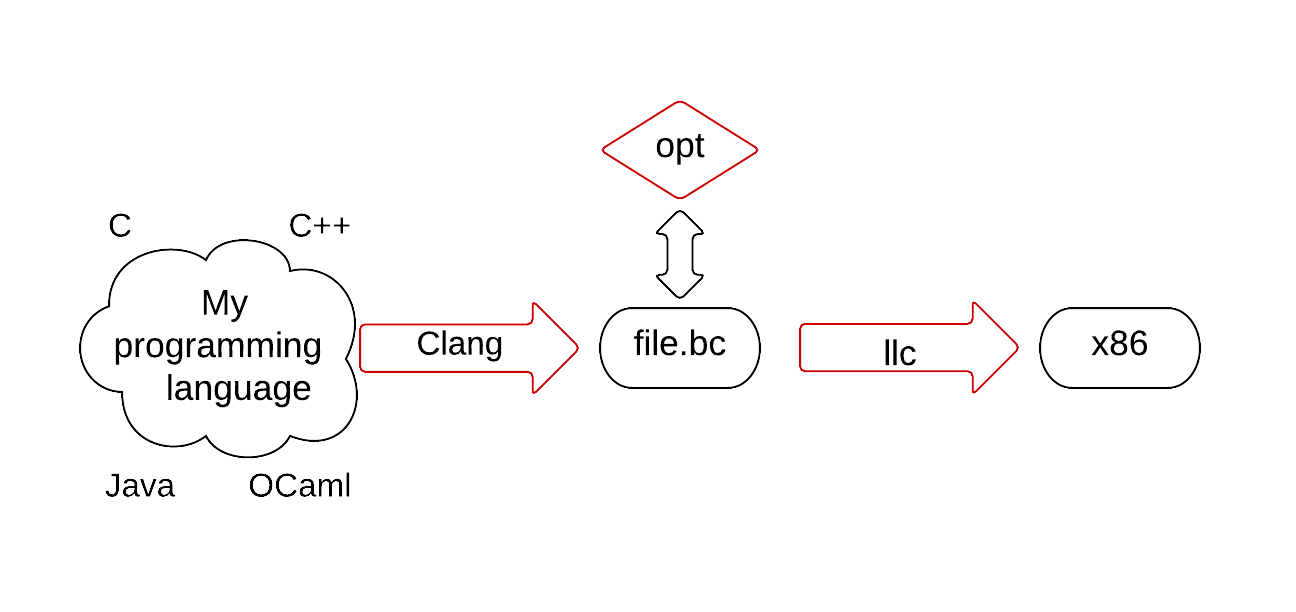
\includegraphics[width=0.7\linewidth]{llvmintro.PNG}
         \label{Pass}
         \caption{Global view of LLVM use}
        \end{figure}
        \end{itemize}
    \end{frame}

\subsection{LLVM Pass}
    \begin{frame}{LLVM Pass}
    \begin{itemize}
            \item Collection of libraries ready-to-use allowing
code analyses and optimizations. Each analyse or optimization
is called a pass.
            \item Example of pass: Memory allocation, common subexpression elimination ...
        \end{itemize}
        \begin{alertblock}{Remark}
                A pass can be run on a complete code or only on a
portion. This leads to the distinction of various types
of passes. In our case, we will focus on ModulePass
(ran on the whole code) and FunctionPass (ran in functions)
        \end{alertblock}
    \end{frame}


%%%%%%%%%%%%%%%%%%%%%%%%%%%%%%%%%%%%%%%%%%%%%%%%%%%%%%%%%%%%%%%%%%%%%%%%%%%%%
%%%%%%%%%%%%%%%%%%%%%%%%%%%%%%%%%%%%%%%%%%%%%%%%%%%%%%%%%%%%%%%%%%%%%%%%%%%%%
\section{Open Computing Language: Open Standard For Parallel Programming}
\subsection{Definition and Organization}
\begin{frame}{Definition}
\begin{itemize}
\item Framework dedicated to writting C programs executed across multiple heterogeneous platforms
\item OpenCL programs are compiled at runtime
\item Platforms are composed of many compute devices
\item Compute device execute programs: kernels
\item One kernel can be executed in different compute devices
\item One kernel can have multiple memory areas: buffers
\item 1 compute device = many processing elements
\end{itemize}
\end{frame}

\begin{frame}{Hierarchy}
\begin{figure}[ht]
         \center
            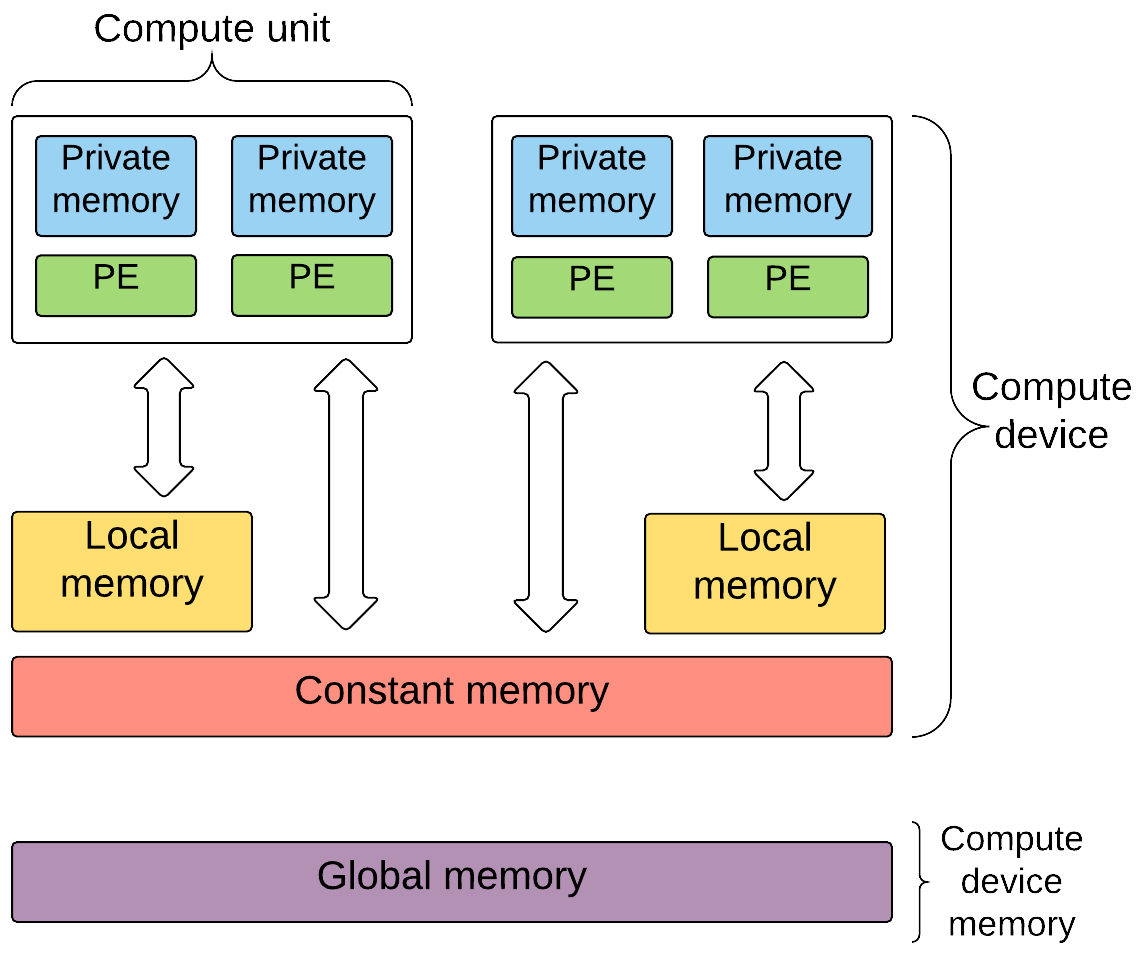
\includegraphics[width=0.55\linewidth]{mem.png}
         \label{Pass}
         \caption{Memory hierarchy in OpenCL}
        \end{figure}
\end{frame}

\subsection{From Runtime to Compile Time}
\begin{frame}{From Runtime to Compile Time}
\begin{itemize}
\item Information about kernel buffers needed (size, access right...) 
\item Known by OpenCL during runtime: communication
\item Link between runtime and compile time
\end{itemize}
\end{frame}




%%%%%%%%%%%%%%%%%%%%%%%%%%%%%%%%%%%%%%%%%%%%%%%%%%%%%%%%%%%%%%%%%%%%%%%%%%%%%%%%%%%%%%%%%%%%%%%%%%
%%%%%%%%%%%%%%%%%%%%%%%%%%%%%%%%%%%%%%%%%%%%%%%%%%%%%%%%%%%%%%%%%%%%%%%%%%%%%%%%%%%%%%%%%%%%%%%%%%
\section{Memory Management Done By LLVM On OpenCL}

\subsection{Organization}
\begin{frame}{Organization}

%begin{itemize}
%\item Compile OpenCL thanks to CLANG for bytecode using SPIR (or Standard Portable Intermediate Representation) 
%\item Generated bytecode used in LLVM with a pass to gather information
%\item Apply testing
%\item Print information to user
%\end{itemize}
\begin{figure}[ht]
    \center
    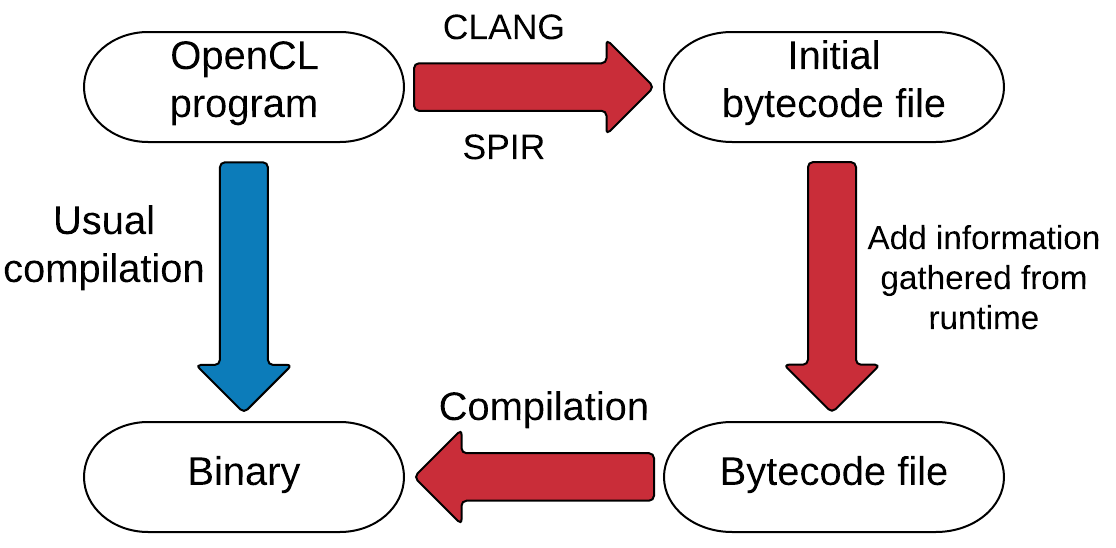
\includegraphics[width=0.6\linewidth]{steps.png}
    \label{Steps}
    \caption{Steps of our work}
\end{figure}

Information of kernels needed. Two options: 
\begin{itemize}
\item Force the user to insert information
\item LLVM pass changing the function signatures at compile time
\end{itemize}
\end{frame}

\subsubsection{Adding arguments}
\begin{frame}[fragile]{Adding arguments}
Function signature before LLVM pass :\\ 
  \lstset{basicstyle=\ttfamily\fontsize{12}{10}\selectfont}
  \begin{lstlisting}[language=C]
define cc76 void @addition(<2 x float> %alpha, 
float addrspace(1)* nocapture %x,
float addrspace(1)* nocapture %y) nounwind 
{/*Body of the function*/}
  \end{lstlisting}
  
Function signature after LLVM pass :\\
  \lstset{basicstyle=\ttfamily\fontsize{12}{7}\selectfont}
  \begin{lstlisting}[language=C]
define cc76 void @addition(<2 x float> %alpha, 
float addrspace(1)* nocapture %x, 
float addrspace(1)* nocapture %y,
int %size_x, int %size_y) nounwind 
{/*Body of the function*/}
  \end{lstlisting}
\end{frame}

\begin{frame}[fragile]{Complementary Information: Metadata}
  \lstset{basicstyle=\ttfamily\fontsize{9.55}{7}\selectfont}
  \begin{lstlisting}[language=C]
!opencl.kernels = !{!0} /*Metadata before LLVM pass*/
!0 = metadata !{void (<2 x float>, float addrspace(1)*, float addrspace(1)*)* @addition, metadata !1, metadata !2, metadata !3, metadata !4, metadata !5}

  \end{lstlisting}
\end{frame}
\begin{frame}[fragile]{Complementary Information: Metadata}
  \lstset{basicstyle=\ttfamily\fontsize{9.55}{7}\selectfont}
  \begin{lstlisting}[language=C]
!opencl.kernels = !{!0} /*Metadata before LLVM pass*/
!0 = metadata !{void (<2 x float>, float addrspace(1)*, float addrspace(1)*)* @addition, metadata !1, metadata !2, metadata !3, metadata !4, metadata !5}

!1 = metadata !{metadata !"kernel_arg_addr_space", i32 0, i32 1, i32 1}
  \end{lstlisting}
\end{frame}
\begin{frame}[fragile]{Complementary Information: Metadata}
  \lstset{basicstyle=\ttfamily\fontsize{9.55}{7}\selectfont}
  \begin{lstlisting}[language=C]
!opencl.kernels = !{!0} /*Metadata before LLVM pass*/
!0 = metadata !{void (<2 x float>, float addrspace(1)*, float addrspace(1)*)* @addition, metadata !1, metadata !2, metadata !3, metadata !4, metadata !5}

!1 = metadata !{metadata !"kernel_arg_addr_space", i32 0, i32 1, i32 1}

!2 = metadata !{metadata !"kernel_arg_access_qual", metadata !"none", metadata !"none", metadata !"none"}
  \end{lstlisting}
\end{frame}
\begin{frame}[fragile]{Complementary Information: Metadata}
  \lstset{basicstyle=\ttfamily\fontsize{9.55}{7}\selectfont}
  \begin{lstlisting}[language=C]
!opencl.kernels = !{!0} /*Metadata before LLVM pass*/
!0 = metadata !{void (<2 x float>, float addrspace(1)*, float addrspace(1)*)* @addition, metadata !1, metadata !2, metadata !3, metadata !4, metadata !5}

!1 = metadata !{metadata !"kernel_arg_addr_space", i32 0, i32 1, i32 1}

!2 = metadata !{metadata !"kernel_arg_access_qual", metadata !"none", metadata !"none", metadata !"none"}

!3 = metadata !{metadata !"kernel_arg_type", metadata !"float2", metadata !"float*", metadata !"float*"}
  \end{lstlisting}
\end{frame}
\begin{frame}[fragile]{Complementary Information: Metadata}
  \lstset{basicstyle=\ttfamily\fontsize{9.55}{7}\selectfont}
  \begin{lstlisting}[language=C]
!opencl.kernels = !{!0} /*Metadata before LLVM pass*/
!0 = metadata !{void (<2 x float>, float addrspace(1)*, float addrspace(1)*)* @addition, metadata !1, metadata !2, metadata !3, metadata !4, metadata !5}

!1 = metadata !{metadata !"kernel_arg_addr_space", i32 0, i32 1, i32 1}

!2 = metadata !{metadata !"kernel_arg_access_qual", metadata !"none", metadata !"none", metadata !"none"}

!3 = metadata !{metadata !"kernel_arg_type", metadata !"float2", metadata !"float*", metadata !"float*"}

!4 = metadata !{metadata !"kernel_arg_type_qual", metadata !"", metadata !"const", metadata !""}
  \end{lstlisting}
\end{frame}
\begin{frame}[fragile]{Complementary Information: Metadata}
  \lstset{basicstyle=\ttfamily\fontsize{9.55}{7}\selectfont}
  \begin{lstlisting}[language=C]
!opencl.kernels = !{!0} /*Metadata before LLVM pass*/
!0 = metadata !{void (<2 x float>, float addrspace(1)*, float addrspace(1)*)* @addition, metadata !1, metadata !2, metadata !3, metadata !4, metadata !5}

!1 = metadata !{metadata !"kernel_arg_addr_space", i32 0, i32 1, i32 1}

!2 = metadata !{metadata !"kernel_arg_access_qual", metadata !"none", metadata !"none", metadata !"none"}

!3 = metadata !{metadata !"kernel_arg_type", metadata !"float2", metadata !"float*", metadata !"float*"}

!4 = metadata !{metadata !"kernel_arg_type_qual", metadata !"", metadata !"const", metadata !""}

!5 = metadata !{metadata !"kernel_arg_base_type", metadata !"float2", metadata !"float*", metadata !"float*"}
  \end{lstlisting}
\end{frame}



\begin{frame}[fragile]{Complementary Information: Metadata}

Metada before LLVM pass:
\lstset{basicstyle=\ttfamily\fontsize{12}{7}\selectfont}
\begin{lstlisting}[language=C]
  !3 = metadata !{metadata !"kernel_arg_type", metadata !"float2", metadata !"float*", metadata !"float*"}
  \end{lstlisting}  

Metadata after LLVM pass:
\lstset{basicstyle=\ttfamily\fontsize{12}{7}\selectfont}
\begin{lstlisting}[language=C]
!3 = metadata !{metadata !"kernel_arg_type", metadata !"float2", metadata !"float*", metadata !"float*", metadata !"int", metadata !"int"}
  \end{lstlisting}
  
\end{frame}

\subsection{Memory Access Testing}

\subsubsection{Aliasing}
\begin{frame}{Aliasing}
\begin{figure}[ht]
         \center
            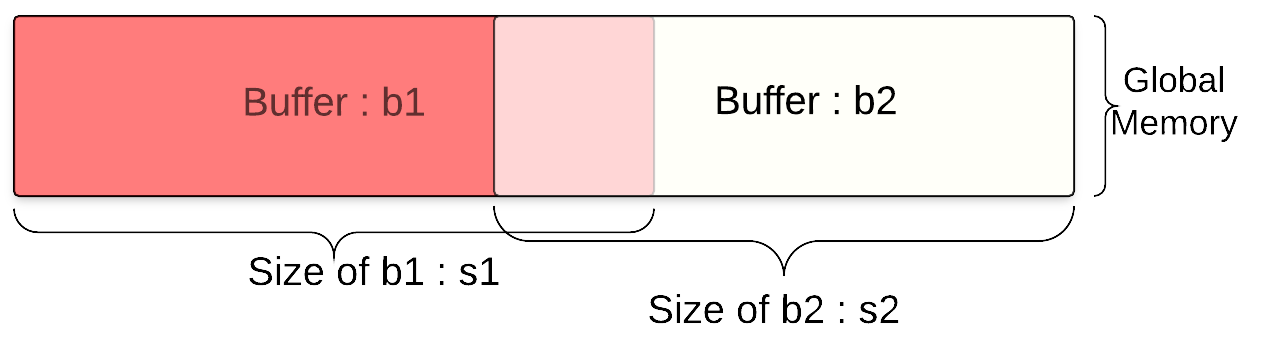
\includegraphics[width=0.7\linewidth]{alias.png}
         \label{Pass}
         \caption{Example of aliasing}
        \end{figure}
\end{frame}

\subsubsection{Out Of Bound}
\begin{frame}{Out Of Bound}
\begin{figure}[ht]
         \center
            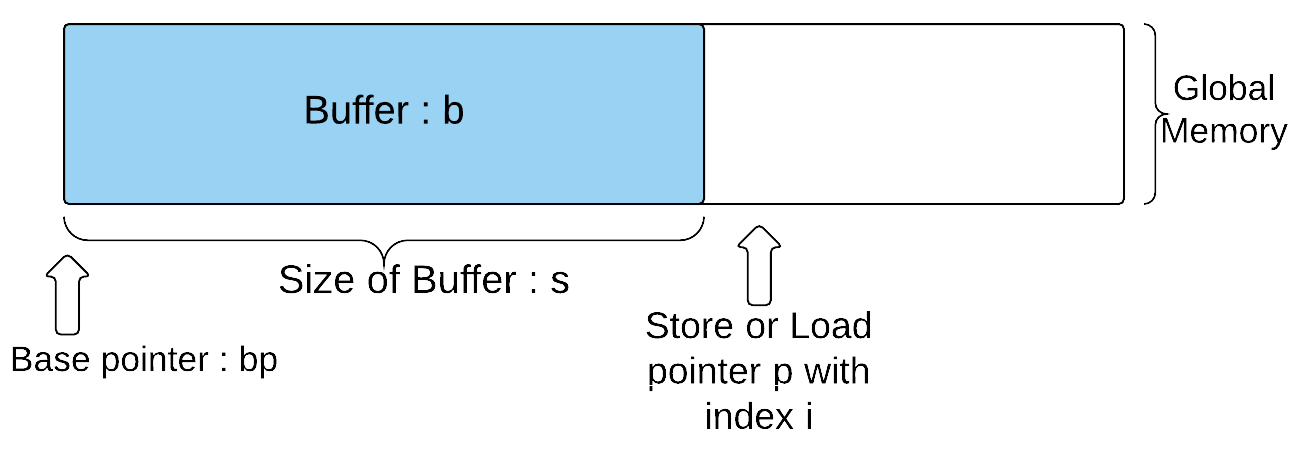
\includegraphics[width=0.7\linewidth]{OFB.png}
         \label{Pass}
         \caption{Example of out-of-bound memory access}
        \end{figure}
\end{frame}


%%%%%%%%%%%%%%%%%%%%%%%%%%%%%%%%%%%%%%%%%%%%%%%%%%%%%%%%%%%%%%%%%%%%%%%%%%%%%%%%%%%%%%%%%%%%%%%%%%
%%%%%%%%%%%%%%%%%%%%%%%%%%%%%%%%%%%%%%%%%%%%%%%%%%%%%%%%%%%%%%%%%%%%%%%%%%%%%%%%%%%%%%%%%%%%%%%%%%
\section{Conclusion}
\begin{frame}{Conclusion}
Future work:
\begin{itemize}
\item Function call using buffers as arguments inside kernel functions
\item Access flag testing
\item Concurrent memory access
\end{itemize}

Application:
\begin{itemize}
\item Created to overcome memory management problem
\item Next big step: Detecting Direct Memory Access races
\end{itemize}
\end{frame}

\subsection{End}
\begin{frame}{End}
\center
Thank you for your attention !
\end{frame}
\end{document}


